%----------------------------------------------------------------------------------------
%	PACKAGES AND OTHER DOCUMENT CONFIGURATIONS
%----------------------------------------------------------------------------------------
\documentclass[a4paper,11pt]{article}

%Include Packages
%----------------------------------------------------
\usepackage{../Header/KaTeX_LabReport}
\usepackage{lipsum}
% Note: 
% The input command is equivalent to copy-paste the content of the file
% into the current file.

\renewcommand{\thesection}{\Roman{section}} 
\titleformat{\section}[display]%command shape
    {\Huge}%format
    {
        \newpage
        \setlength\fboxsep{0pt}
        \color{gray} \fontsize{20}{5}\selectfont\chaptername\ \thesection
    }%label
    {0pt}{}{}
\titlespacing*{\section}{0pt}{0pt}{20pt}
\renewcommand{\thesubsection}{\thesection: \Roman{subsection}}
\renewcommand{\thesubsubsection}{\thesubsection. \roman{subsubsection}}
\renewcommand{\thesubsection}{\Roman{subsection}}
\titleformat{\subsection}
    {\bfseries\Large}%format
    {\huge\textnormal{\thesubsection}}%label
    {12pt}{}{}

\usepackage{sectsty}
    \sectionfont{\LARGE}
    \subsectionfont{\large}
    \subsubsectionfont{\large}
    \paragraphfont{\large}
\usepackage{titletoc}
    \titlecontents{}[1em]{\addvspace{1pc}\bfseries}      {\contentslabel{3em}}{}
    {\titlerule*[0.3pc]{.}\contentspage}

\usepackage{tocloft}% http://ctan.org/pkg/tocloft
\setlength\cftsecnumwidth{6em}

\renewcommand{\thesubsubsection}{\thesubsection: \roman{subsubsection}}
\titlespacing{\subsubsection}{0pt}{15pt}{5pt}

%Hyperlink Setting
%----------------------------------------------------
\hypersetup{hidelinks,
	colorlinks=true,
	allcolors=black,
	pdfstartview=Fit,
	breaklinks=true
}

% \includeonly{
%     Experiment_01/Lab1_Main,
%     Experiment_02/Lab2_Main,
%     Experiment_07/Lab7_Main,
% }

\begin{document}
%----------------------------------------------------------------------------------------
%	FRONT MATTER
%----------------------------------------------------------------------------------------
% Cover
\thispagestyle{empty}
\begin{titlepage}
    % Warning Filter
    \WarningFilter[latex]{latexfont}{Some font shapes}
    \WarningFilter[latex]{tex}{Underfull \hbox}
    \ActivateWarningFilters[latex]

	%\hspace{0.05\textheight} % Whitespace between the vertical line and title page text
    \parbox{1\textwidth}{ % Paragraph box for holding the title page text, adjust the width to move the title page left or right on the page
		{\Huge\bfseries EIE420 Assignment II \\[0.15\baselineskip] 
        Gray Scale Histrogram}\\[0.15\baselineskip] % Title
		\rule{1\textwidth}{1pt} % Vertical line
        {\Large\textit{Report of EIE420, Digital Image Processing Assignment}}
        \newline
    }
    \parbox{1\textwidth}{
        \vspace{1\baselineskip}
        \large
        Source Code of this assignment could be found at:\newline
        \url{https://github.com/ZeppelinSCB/EIE420-Digital_Image_Processing}
        \newline
    }
    \vspace{100pt} % Whitespace between the title block and the publisher
    \parbox{1\textwidth}{
        {\large by}\\[1.5\baselineskip]
        {\rule[1pt]{200pt}{1pt}} \\[1.25pt]
        {\huge\textsc{Pengrui K. Tong}
            %\begin{CJK*}{UTF8}{bsmi}\Large (湯鵬睿)\end{CJK*}
            }\\
        {\large{Student No: 1220031811}} \\
        \large from EIE420 D1, \newline
        Faculty of Innovation Engeneering, \newline
        Universidade de Ciência e Tecnologia de Macau
    }
		

    \vspace*{\fill}
		Apr 6, 2025 \newline 
        (Coloane, Macao, SAR)
        \vspace{0.7\baselineskip}\newline
        %
\includegraphics[width = 40mm]{MUIT_BlueGold.png}\newline
        
\includegraphics[width = 40mm]{../Header/MUIT_origin.png}\par
        {\small Cover Design by Karl Tong}\\[0.25pt]
        {\small This report is a part of the result for}
        {\small EIE420~Digital~Image~Processing in U.C.T.M}\\[0.25pt]
        {\small \copyright 2025 Pengrui Tong}
\end{titlepage}
\blankpage

% Table of Contents
\tableofcontents
\blankpage

\section{Problem Statement}
A grayscale histogram represents the distribution of pixel intensity levels in an image, ranging from black to white. By analyzing the histogram, one can adjust brightness, detect objects, and improve image quality for better visualization and analysis.
\\
\subsection{Objective}
    In this experiment, we want to implement two algorithm relate to grayscale histogram. First the algorithm that calculate the histogram from a given image; the second can do the histogram equalization for given grayscale or RGB image.\\

\section{Procedure}
In this experiment, I will implemented two functions. The first function is to calculate the histogram of an image, and the second function is to perform histogram equalization for images. The first function will be used as a helper function for the second one.\\

\subsection{Design of the Histogram calculate function}
\subsubsection{Function description}
This function take a 2D or 3D matrix as input, and return a 1-D matrix with the same size as the number of pixel intensity levels. The function will count the number of pixels for each intensity level, and return the result in a 1-D matrix.\\

In order to deal with input of different types, the function first check the input dimension, and will assumen the input is a grayscale image if the input is 2D matrix. If the input is a 3D matrix, the function will convert it to HSV image and extract the Value channel, and scale it to 8-bit unsigned interger.\\
\begin{enumerate}
    \item Input check:
        \begin{enumerate}
            \item Determine the dimensions of the input image (img).
            \item If the image is RGB (3 dimensions), convert it to HSV and extract the Value channel, then scale it to 8-bit (0-255).
            \item If the image is grayscale (2 dimensions), directly use it.
            \item If the image is neither, throw an error.
        \end{enumerate}

    \item Compute Histogram:
        \begin{enumerate}
            \item Initialize a histogram array of size 256.
            \item Traverse the image matrix and count add the count of each pixel to the corresponding index in the histogram array.
        \end{enumerate}

    \item Return the output array.
\end{enumerate}
\subsubsection{Designed IO}
\subsubsection*{Input}
\textbf{image}: \\
Image input. An uint8 format matrix with three dimention.
\subsubsection*{Output}
\textbf{imOut}: \\
Output image. An uint8 format matrix with three dimention, and contains the original image as well as the splited channel in the order of the channel's index.

\subsection{Design of the Histogram Equalization function (Grayscale and Colored)}
\subsubsection{Function description}
This function will take a 2D or 3D matrix as input, and return a matrix with same dimensions and size as the input image. The function will perform histogram equalization on the input image, and return the equalize image\\

Similar to the histogram function, this function also check the input image type. And convert the image to grayscale depending on the input type.\\

\begin{figure}[H]
    \centering
    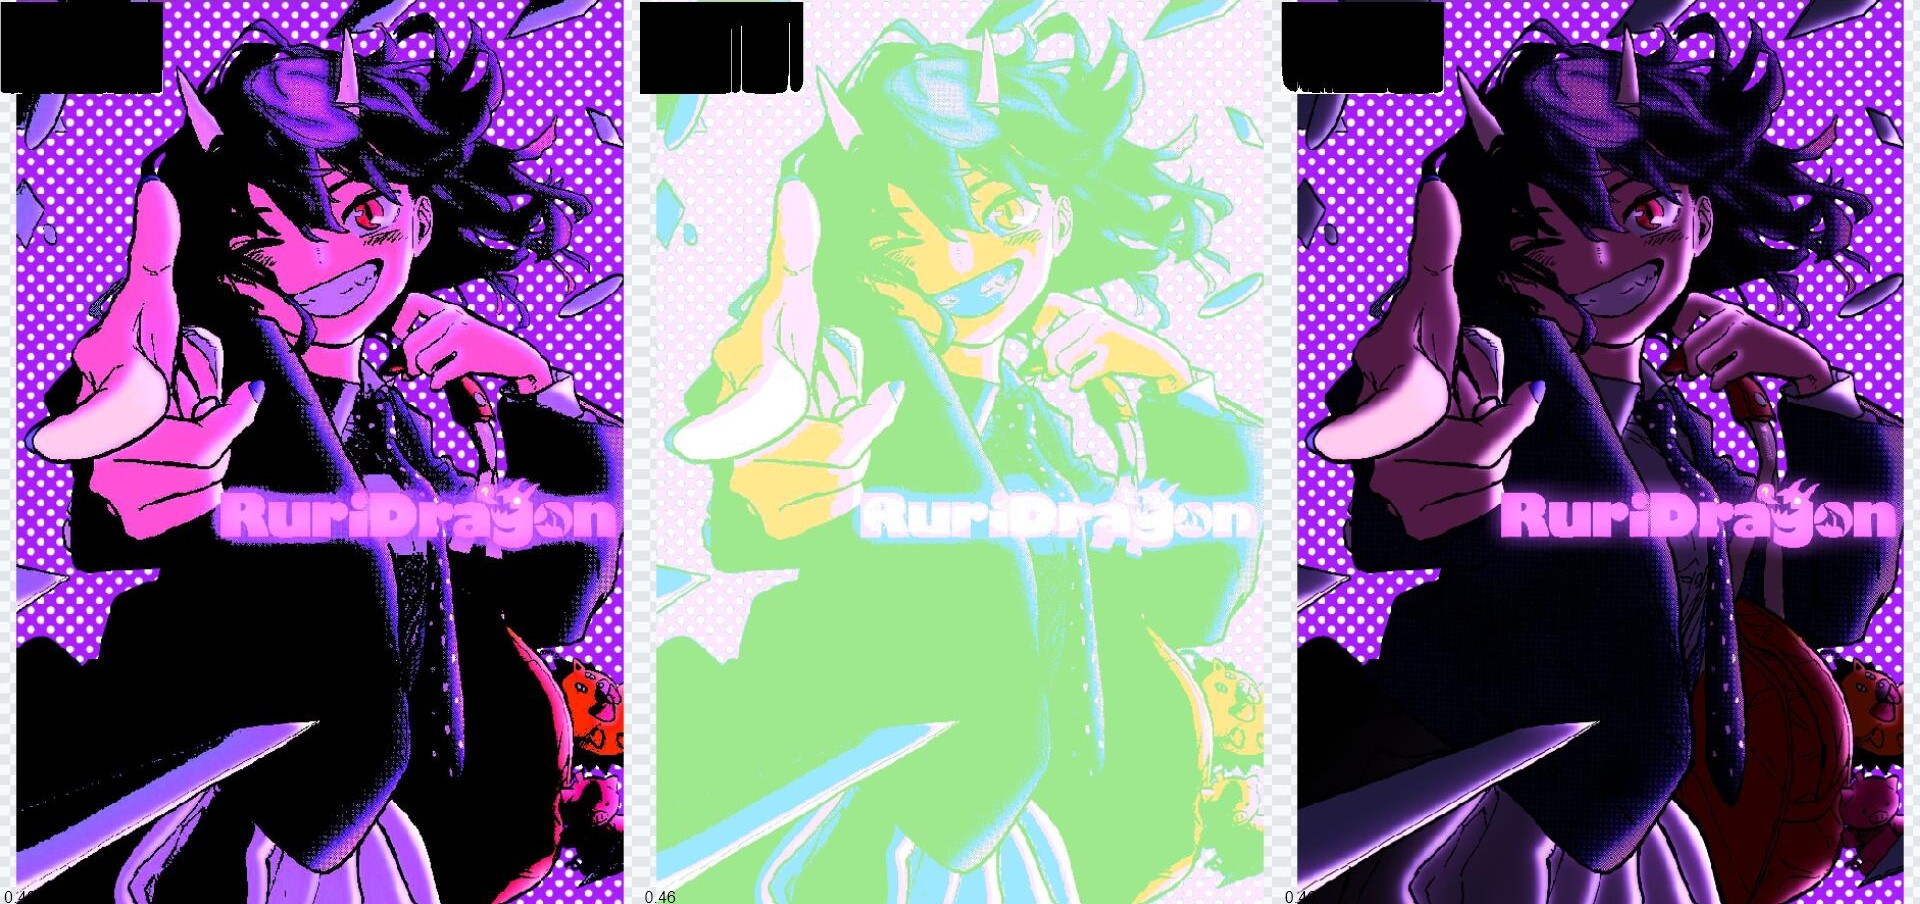
\includegraphics[width=0.8\linewidth]{Demo3-InccoorectlyEqualized.jpg}
    \caption{Equalization done on each channel of RGB image}
    \label{pic:Mistake1}
\end{figure}

Worth noting that, we perform histogram equalization on the Value channel of the HSV image, and then convert it back to RGB. The result is shown in the leftmost image in figure \ref{pic:Mistake1}. Otherwise, if we directly perform the equalization on each channel of RGB image, the result will be distorted, as shown in the center image of figure \ref{pic:Mistake1}. The original is shown on the right for reference.\\
\begin{enumerate}
    \item Input check
    \begin{enumerate}
        \item Determine the size and dimensions of the input image using \texttt{size(img)}. Identify if the image is grayscale (2D) or RGB (3D) using \texttt{length(imgSize)}.
        \item For RGB images (3D):
        \begin{itemize}
            \item Convert the image to HSV color space using \texttt{rgb2hsv(img)}.
            \item Extract the \textquotedblleft Value\textquotedblright\ channel and scale it to 8-bit using \texttt{uint8(imgHSV(:,:,3) * 255)}.
        \end{itemize}
        \item For Grayscale images (2D):
        \begin{itemize}
            \item Directly convert the image to 8-bit format using \texttt{uint8(img)}.
        \end{itemize}
        \item Raise an error if the image is neither 2D nor 3D, indicating invalid input.
    \end{enumerate}
\end{enumerate}

    \begin{enumerate}
        \item Compute the histogram of the image using \texttt{hist\_int(img)}, which returns a 1-by-256 array.
        \item Calculate the Cumulative Distribution Function (CDF):
        \begin{itemize}
            \item Compute the cumulative sum of the histogram with \texttt{cumsum(hist)}.
            \item Normalize the CDF by dividing it by \texttt{cdf(end)} to ensure values range from 0 to 1.
            \item Scale the CDF to the range [0, 255] using \texttt{cdf * 255}, creating a mapping for intensity values.
        \end{itemize}
        \item Apply histogram equalization:
        \begin{itemize}
            \item Map original intensity values to new values using the scaled CDF with \texttt{cdfW(img8b + 1)}.
        \end{itemize}
        \item Reconstruct the processed image:
        \begin{itemize}
            \item For \textbf{RGB images}, update the \textquotedblleft Value\textquotedblright\ channel with equalized values and convert back to RGB using \texttt{hsv2rgb(imgHSV)}. Store the result in \texttt{imgEql}.
            \item For \textbf{Grayscale images}, convert the equalized image to 8-bit format and store it as \texttt{imgEql}.
        \end{itemize}
    \end{enumerate}


\section{Source Code}
\subsection{Main Program Code}
\lstset{language = Matlab}
    \begin{lstlisting}[basicstyle=\tiny]clc;
        IMAGE = 'Suletta and Miorine';
        FOLDER = 'work/';
        PATH = append(FOLDER,IMAGE,'.jpg');
        I = imread(PATH);
        
        subplot(2,3,1)
        imshow(I);
        title('Original Image');
        
        subplot(2,3,2)
        title('Gray Scale of the Original');
        gHist = hist_int(I);
        subplot(2,3,3)
        bar(gHist);
        title('Histogram of Original Image');
        
        % Equalization
        subplot(2,3,4)
        imgEql = hist_eql(I);
        imshow(imgEql);
        title('Equalized Image');
        imwrite(imgEql,append(FOLDER,IMAGE,'-Eql.jpg'));
        size(imgEql);
        
        subplot(2,3,5)
        title('Gray Scale of the Equalized');
        eHist = hist_int(imgEql);
        subplot(2,3,6)
        bar(eHist);
        title('Histogram of Equalized Image');
\end{lstlisting}

\subsection{Code for Histogram calculation}
\lstset{language = Matlab}
    \begin{lstlisting}[basicstyle=\tiny]
        function his = hist_int(img)
        imgSize = size(img);
        dimation = length(imgSize);
        if dimation == 3 %Assume input is RGB format
            imgHSV = rgb2hsv(img);
            img16b = uint8(imgHSV(:,:,3).*255);
            imshow(img16b)
        elseif dimation == 2 %If dimention is 2, Assume Grey image
            img16b = uint8(img);
        else
            error('Input image must be either a gray image or a RGB image');
        end
    
        his = zeros(1,256);
        m = imgSize(1);
        n = imgSize(2);
        for i = 1:m
            for j = 1:n
                his(img16b(i,j)+1) = his(img16b(i,j)+1) + 1;
            end
        end
    end
\end{lstlisting}

\subsection{Code for Histogram Equalization}
\lstset{language = Matlab}
    \begin{lstlisting}[basicstyle=\tiny]
    function imgEql = hist_eql(img)
        imgSize = size(img);
        dimation = length(imgSize);
        if dimation == 3 %Assume input is RGB format
            imgHSV = rgb2hsv(img);
            img8b = uint8(imgHSV(:,:,3).*255);%Convert double to uint8
        elseif dimation == 2 %If dimention is 2, Assume Grey image
            img8b = uint8(img);
        else
            error('Input image must be either a gray image or a RGB image');
        end
    
        hist = hist_int(img);
        % Cumilative Sum
        cdf = cumsum(hist);
        % Calculate CDF
        cdf = cdf/cdf(end);
        % Scale to 0-255
        cdfW = cdf * 255;
        % Apply the equalization
        grayEql = cdfW(img8b + 1);
        
        if dimation == 3
            imgHSV(:,:,3) = double(grayEql)/255;%apply the equalized image
            imgEql = hsv2rgb(imgHSV);%convert back to RGB
        elseif dimation == 2
            % Convert to uint8
            imgEql = uint8(grayEql);
        end
    end
\end{lstlisting}

\section{Discussion}
\subsection{Sample Program Output}
\begin{figure}[H]
    \centering
    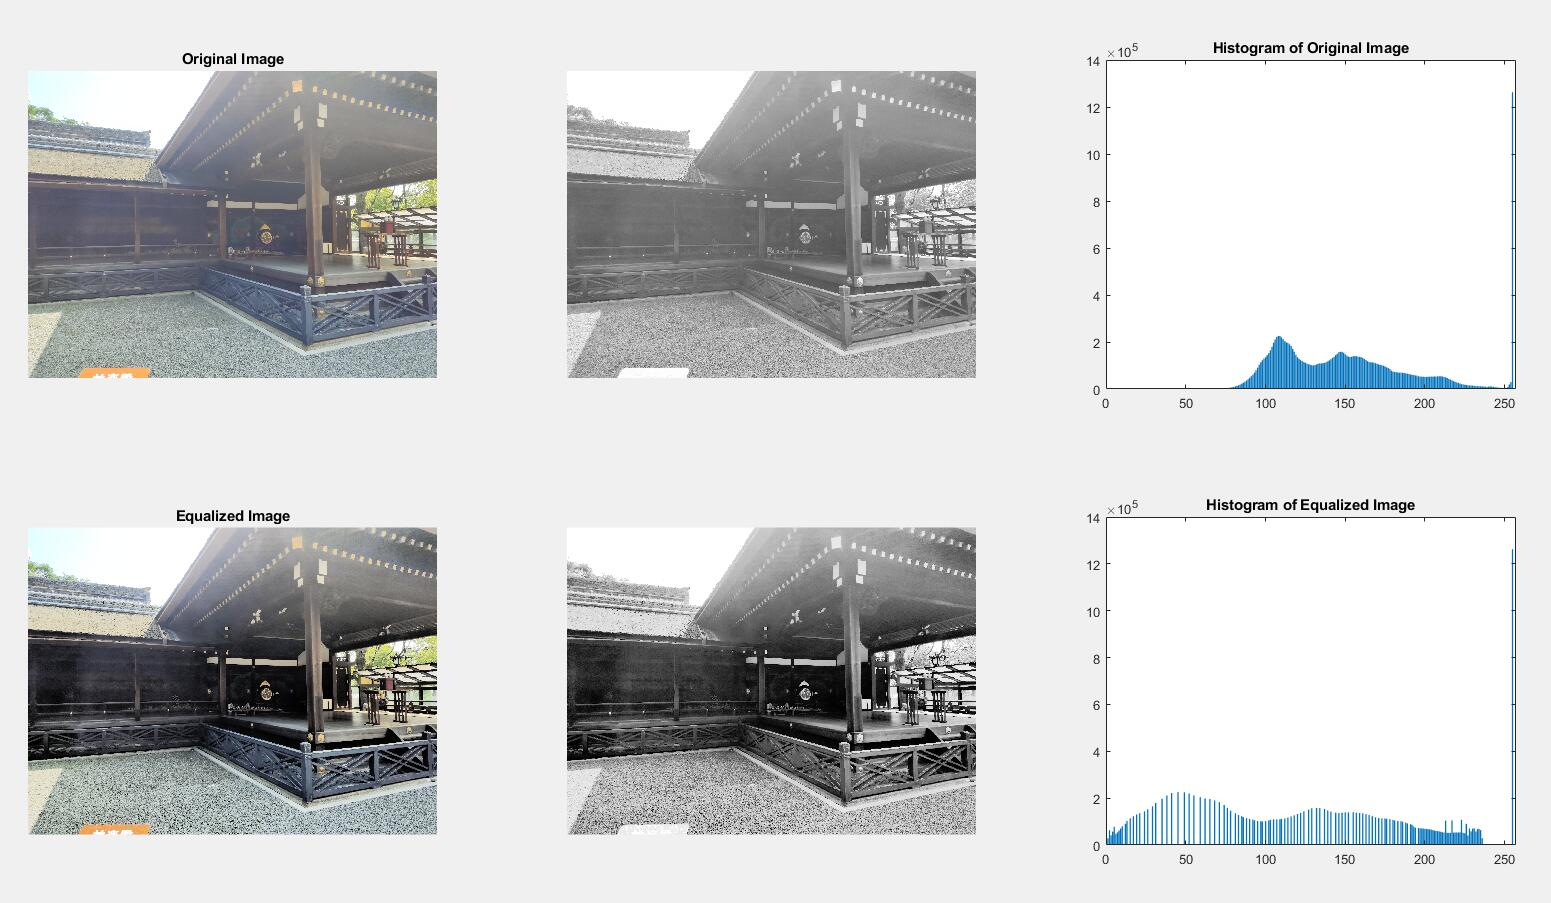
\includegraphics[width=0.8\linewidth]{Demo2-Colored.jpg}
    \caption{Equalization of a colored image}
    \label{pic:Demo_2}
\end{figure}
We test the code multiple times with one image of ginga. The result is shown in figure:\ref{pic:Demo_2}. The Value channel of the converted HSV image and the calculated histogram is provided for reference.\\
\begin{figure}[H]
    \centering
    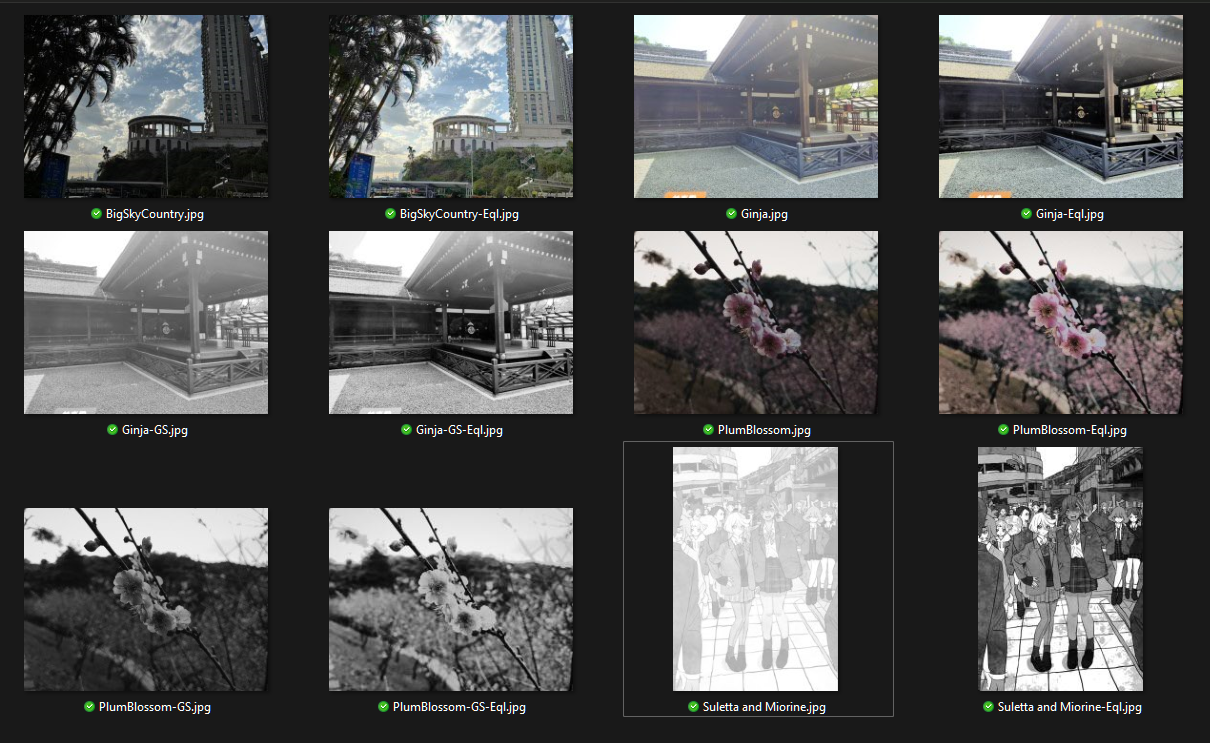
\includegraphics[width=0.9\linewidth]{Demo_1.png}
    \caption{Series of images before and after equalization}
    \label{pic:Demo_2}
\end{figure}
Then, we reun the code multiple time with different images. Overall, the result is expected. However, we also notice some distortion if the image's histogram is not disctruted enough. We can see that's due the lack of information in the original image, and couldn't be fixed by the algorithm.\\

\section{Conclusion}
In conclusion, the experiment effectively implemented histogram calculation and equalization algorithms, enhancing the contrast of grayscale and RGB images. These functions improved visual quality by transforming image data into a histogram and utilizing the cumulative distribution function for equalization, especially beneficial for images with poor contrast. Despite their success, some limitations appeared in images with insufficient intensity distribution, highlighting the dependence on original image quality. This experiment provided valuable insights into image processing, demonstrating histogram-based methods' potential for improving clarity and offering opportunities for refinement to address specific image types.

\section{References}
No outside sources was referened expect the lecture notes and the matlab official doucumentation.
\end{document}